% !TEX program = xelatex

\documentclass{beamer}
\usepackage[utf8]{inputenc}
\usepackage{xeCJK}
\usepackage{utopia} %font utopia imported
%\usepackage[UTF8,noindent]{ctexcap}
\usepackage{latexsym,amssymb,amsmath,amsbsy,amsopn,amstext,xcolor,multicol}
\usepackage{graphicx,wrapfig,fancybox}
\usetheme{Rochester}
\usecolortheme{default}
 % 衬线字体:Linux Libertine
    % BoldFont 可以选择 Bold 字重或者 Semibold 字重
    % BoldItalicFont 也有对应 BoldFont 的字重选择
    % 这里使用 Semibold 字重
  %   \setmainfont{LinLibertine_R.otf}[
  %     BoldFont = LinLibertine_RZ.otf,
  %     ItalicFont = LinLibertine_RI.otf,
  %     BoldItalicFont = LinLibertine_RZI.otf]
  % % % 无衬线字体:Linux Biolinum
  % \setsansfont{LinBiolinum_R.otf}[
  %     BoldFont = LinBiolinum_RB.otf,
  %     ItalicFont = LinBiolinum_RI.otf,
  %     BoldItalicFont = LinBiolinum_RBO.otf]
  % % 等宽/打印机字体:Linux Libertine Mono
  % \setmonofont{LinLibertine_M.otf}[
  %     BoldFont = LinLibertine_MB.otf,
  %     ItalicFont = LinLibertine_MO.otf,
  %     BoldItalicFont  = LinLibertine_MBO.otf]
  % \setCJKmainfont[ItalicFont={AR PL UKai CN},
  % BoldFont={WenQuanYi Micro Hei}]{IPAMinCho,IPA明朝}
  \setCJKsansfont{WenQuanYi Micro Hei}
  \setCJKmonofont{WenQuanYi Micro Hei Mono}
%------------------------------------------------------------
%This block of code defines the information to appear in the
%Title page
\title[光电中期报告] %optional
{光电子技术实验}

\subtitle{固体激光器的静态特性及调Q技术}

\author[芦, 王] % (optional)
{芦迪 \and 王莘景}

\institute[THU, EE] % (optional)
{

  Department of Electronic Engineering,\\
  Tsinghua University
}

\date[2017.11.8] % (optional)
{\today}

\logo{
\includegraphics[height=1.5cm]{images/thuee-logo.png}}

%End of title page configuration block
%------------------------------------------------------------



%------------------------------------------------------------
%The next block of commands puts the table of contents at the 
%beginning of each section and highlights the current section:

\AtBeginSection[]
{
  \begin{frame}
    \frametitle{目录}
    \tableofcontents[currentsection]
  \end{frame}
}
%------------------------------------------------------------


\begin{document}
%The next statement creates the title page.
\frame{\titlepage}


%---------------------------------------------------------
%This block of code is for the table of contents after
%the title page
\begin{frame}
\frametitle{目录}
\tableofcontents
\end{frame}
%---------------------------------------------------------


\section{实验任务}

%---------------------------------------------------------
%Changing visivility of the text
\begin{frame}
\frametitle{实验任务}

本次实验的实验目的为:
\begin{enumerate}
  \item 掌握固体激光器与调 Q 工作原理
  \item 掌握固体激光器的调节方法,了解谐振腔参数及调节精度对激光器性能的影响
  \item 测量固体激光器的静态输出特性和调Q输出特性
  \item 掌握用于固体激光器调整和测量仪器的使用方法
\end{enumerate}
\end{frame}

\begin{frame}
  \frametitle{实验任务}
为达到以上目的,实验设计了如下任务: \\

\begin{enumerate}
    \item 装调固体激光器使之产生激光,反复调整降低阈值
    \item 测量固体激光器输出-输入能量关系曲线
    \item 观察激光器的静态输出波形,记录其波形与总宽度
    \item 测量固体激光器调Q输出波形,改变输入能量观察输出脉冲个数
    \item 测量固体激光器调Q输出-输入能量关系曲线并分析其特点
    \item 观测谐振腔调制精度对激光器的影响
\end{enumerate}
\end{frame}

%---------------------------------------------------------


%---------------------------------------------------------
%Example of the \pause command
% \begin{frame}
%   \frametitle{实验原理}
% In this slide \pause

% the text will be partially visible \pause

% And finally everything will be there
% \end{frame}
%---------------------------------------------------------

\section{实验原理}

%---------------------------------------------------------
%Highlighting text
\begin{frame}{固体激光器工作原理}
% \frametitle
固体激光器的结构如图:
\begin{figure}
  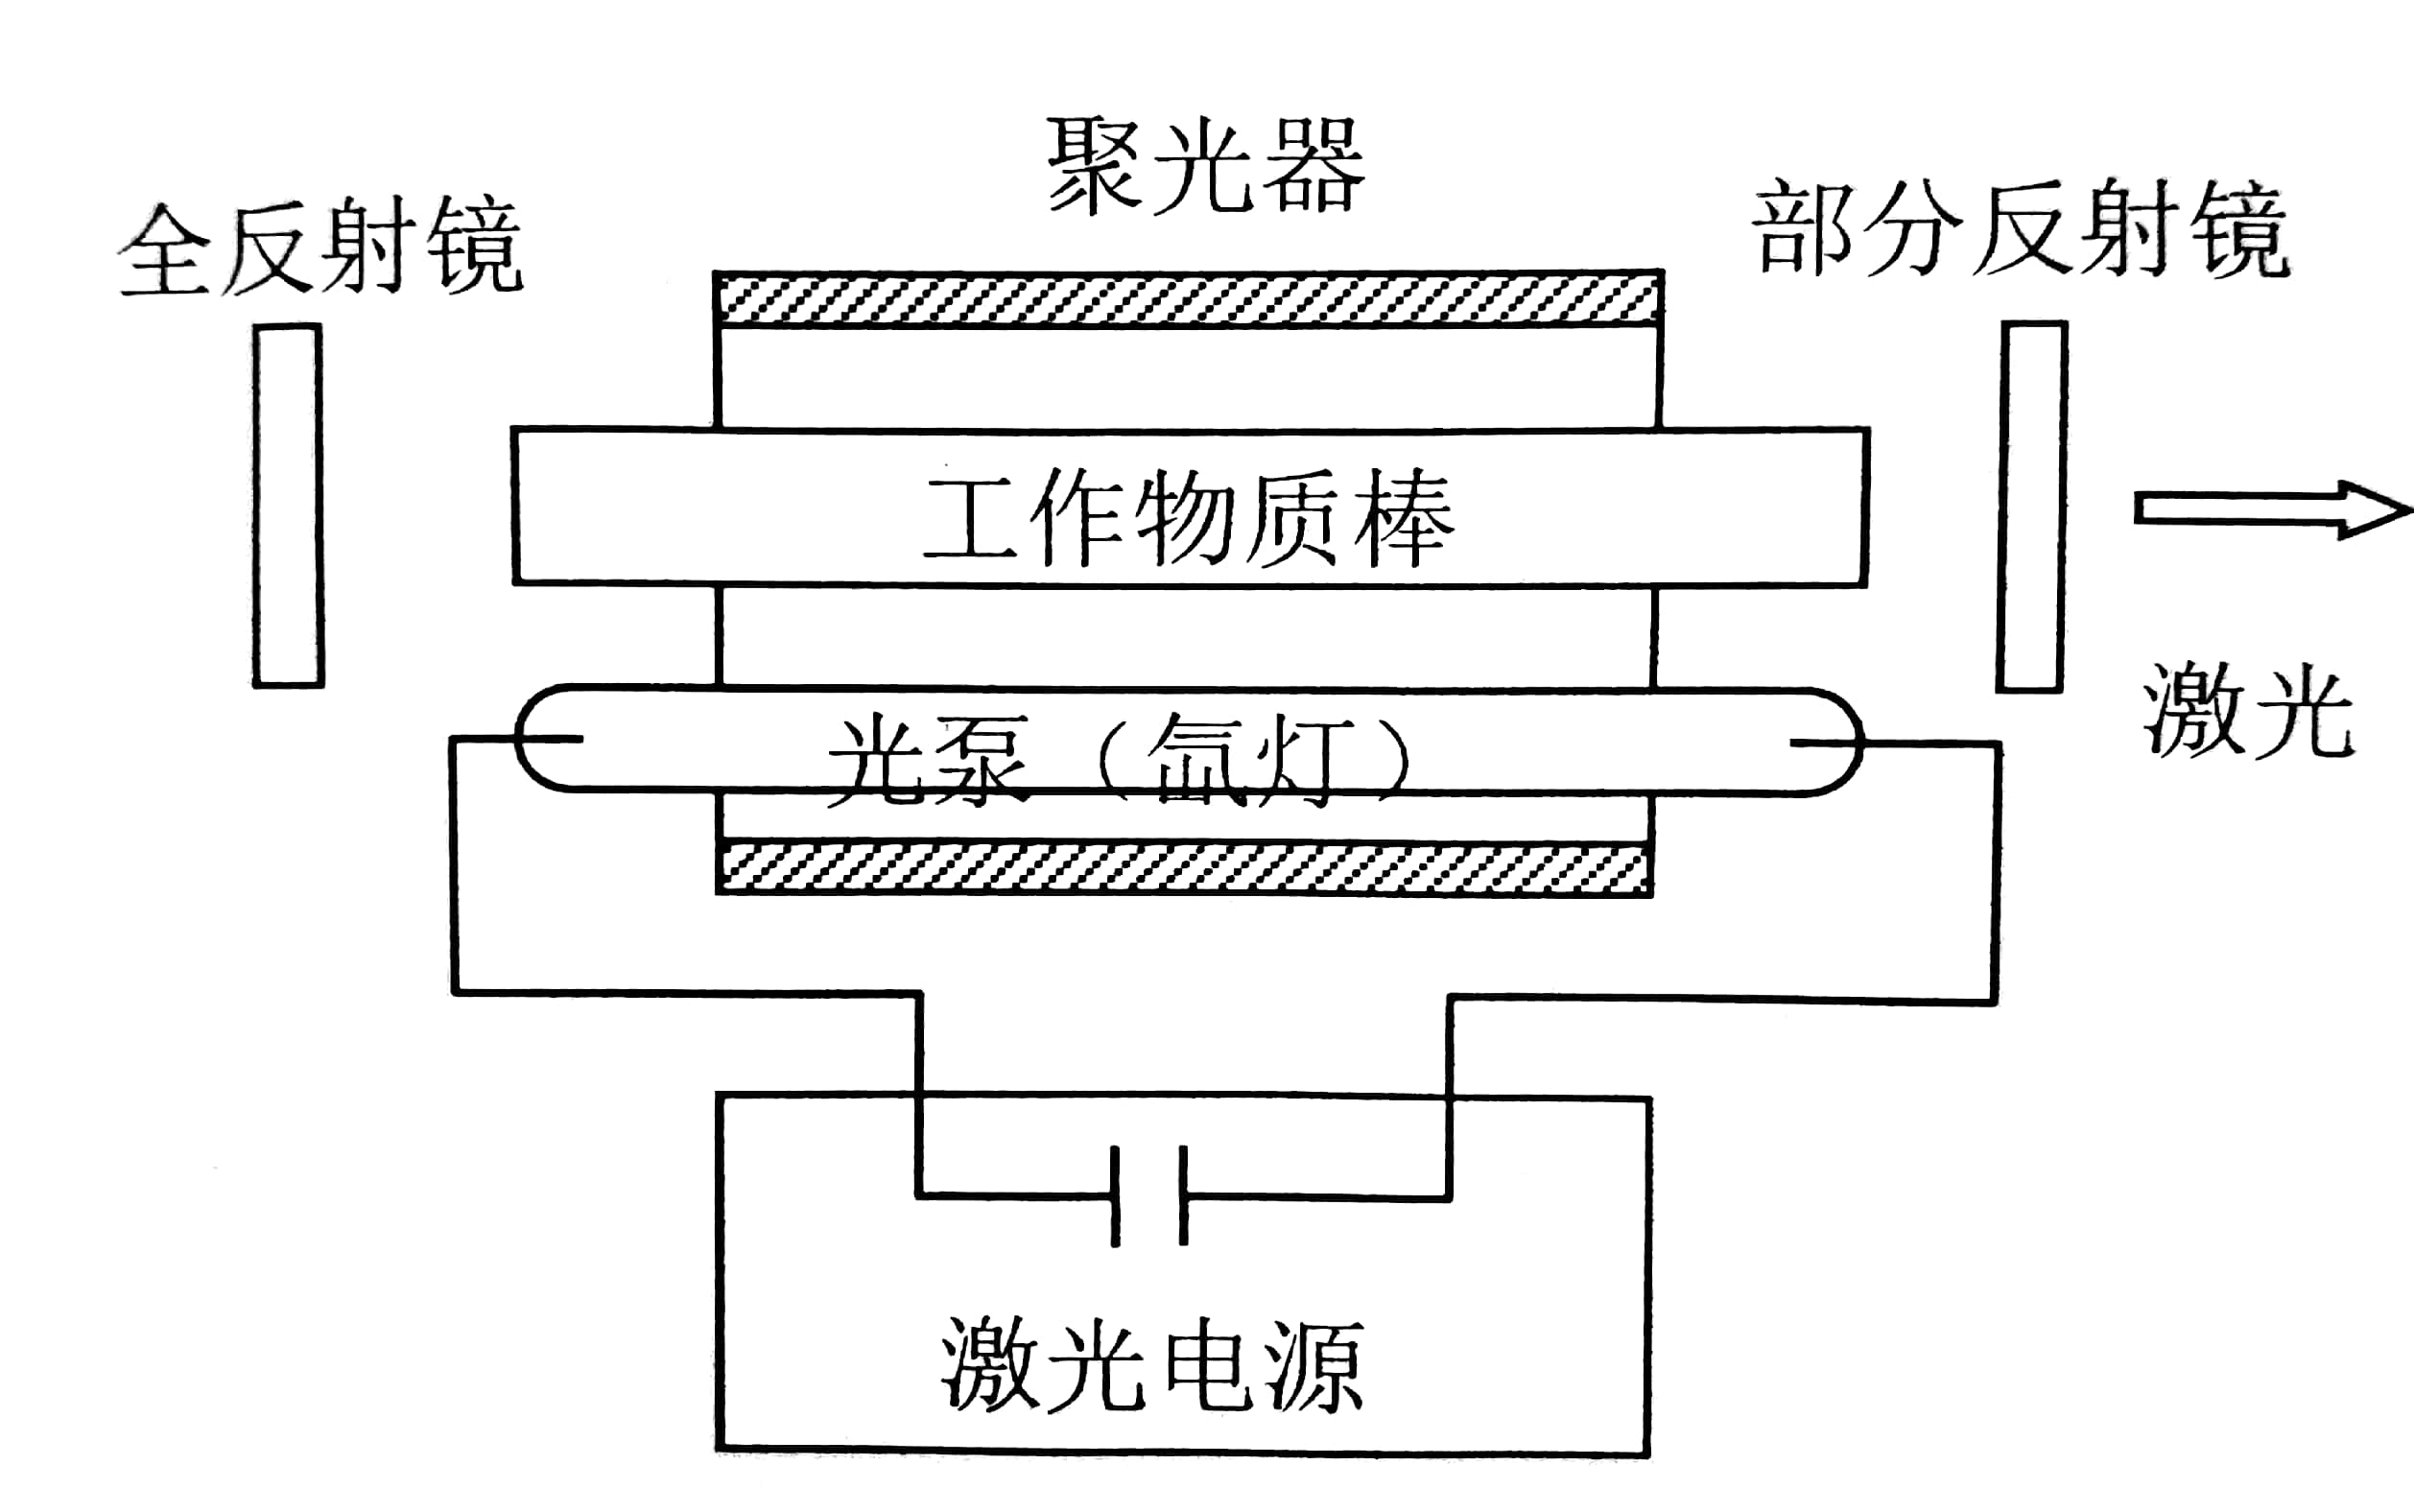
\includegraphics[height=3cm,width=5cm]{images/1.jpg}
  \label{fg1}
\end{figure}
本实验采用的工作物质为 \(\rm Nd:YAG\),激活离子为\(\rm Nd^{3+}\),激光输出波长为\(1.06\mu m\)。
\end{frame}
\begin{frame}{固体激光器工作原理}
  钕离子的能级示意图为:
  \begin{figure}
    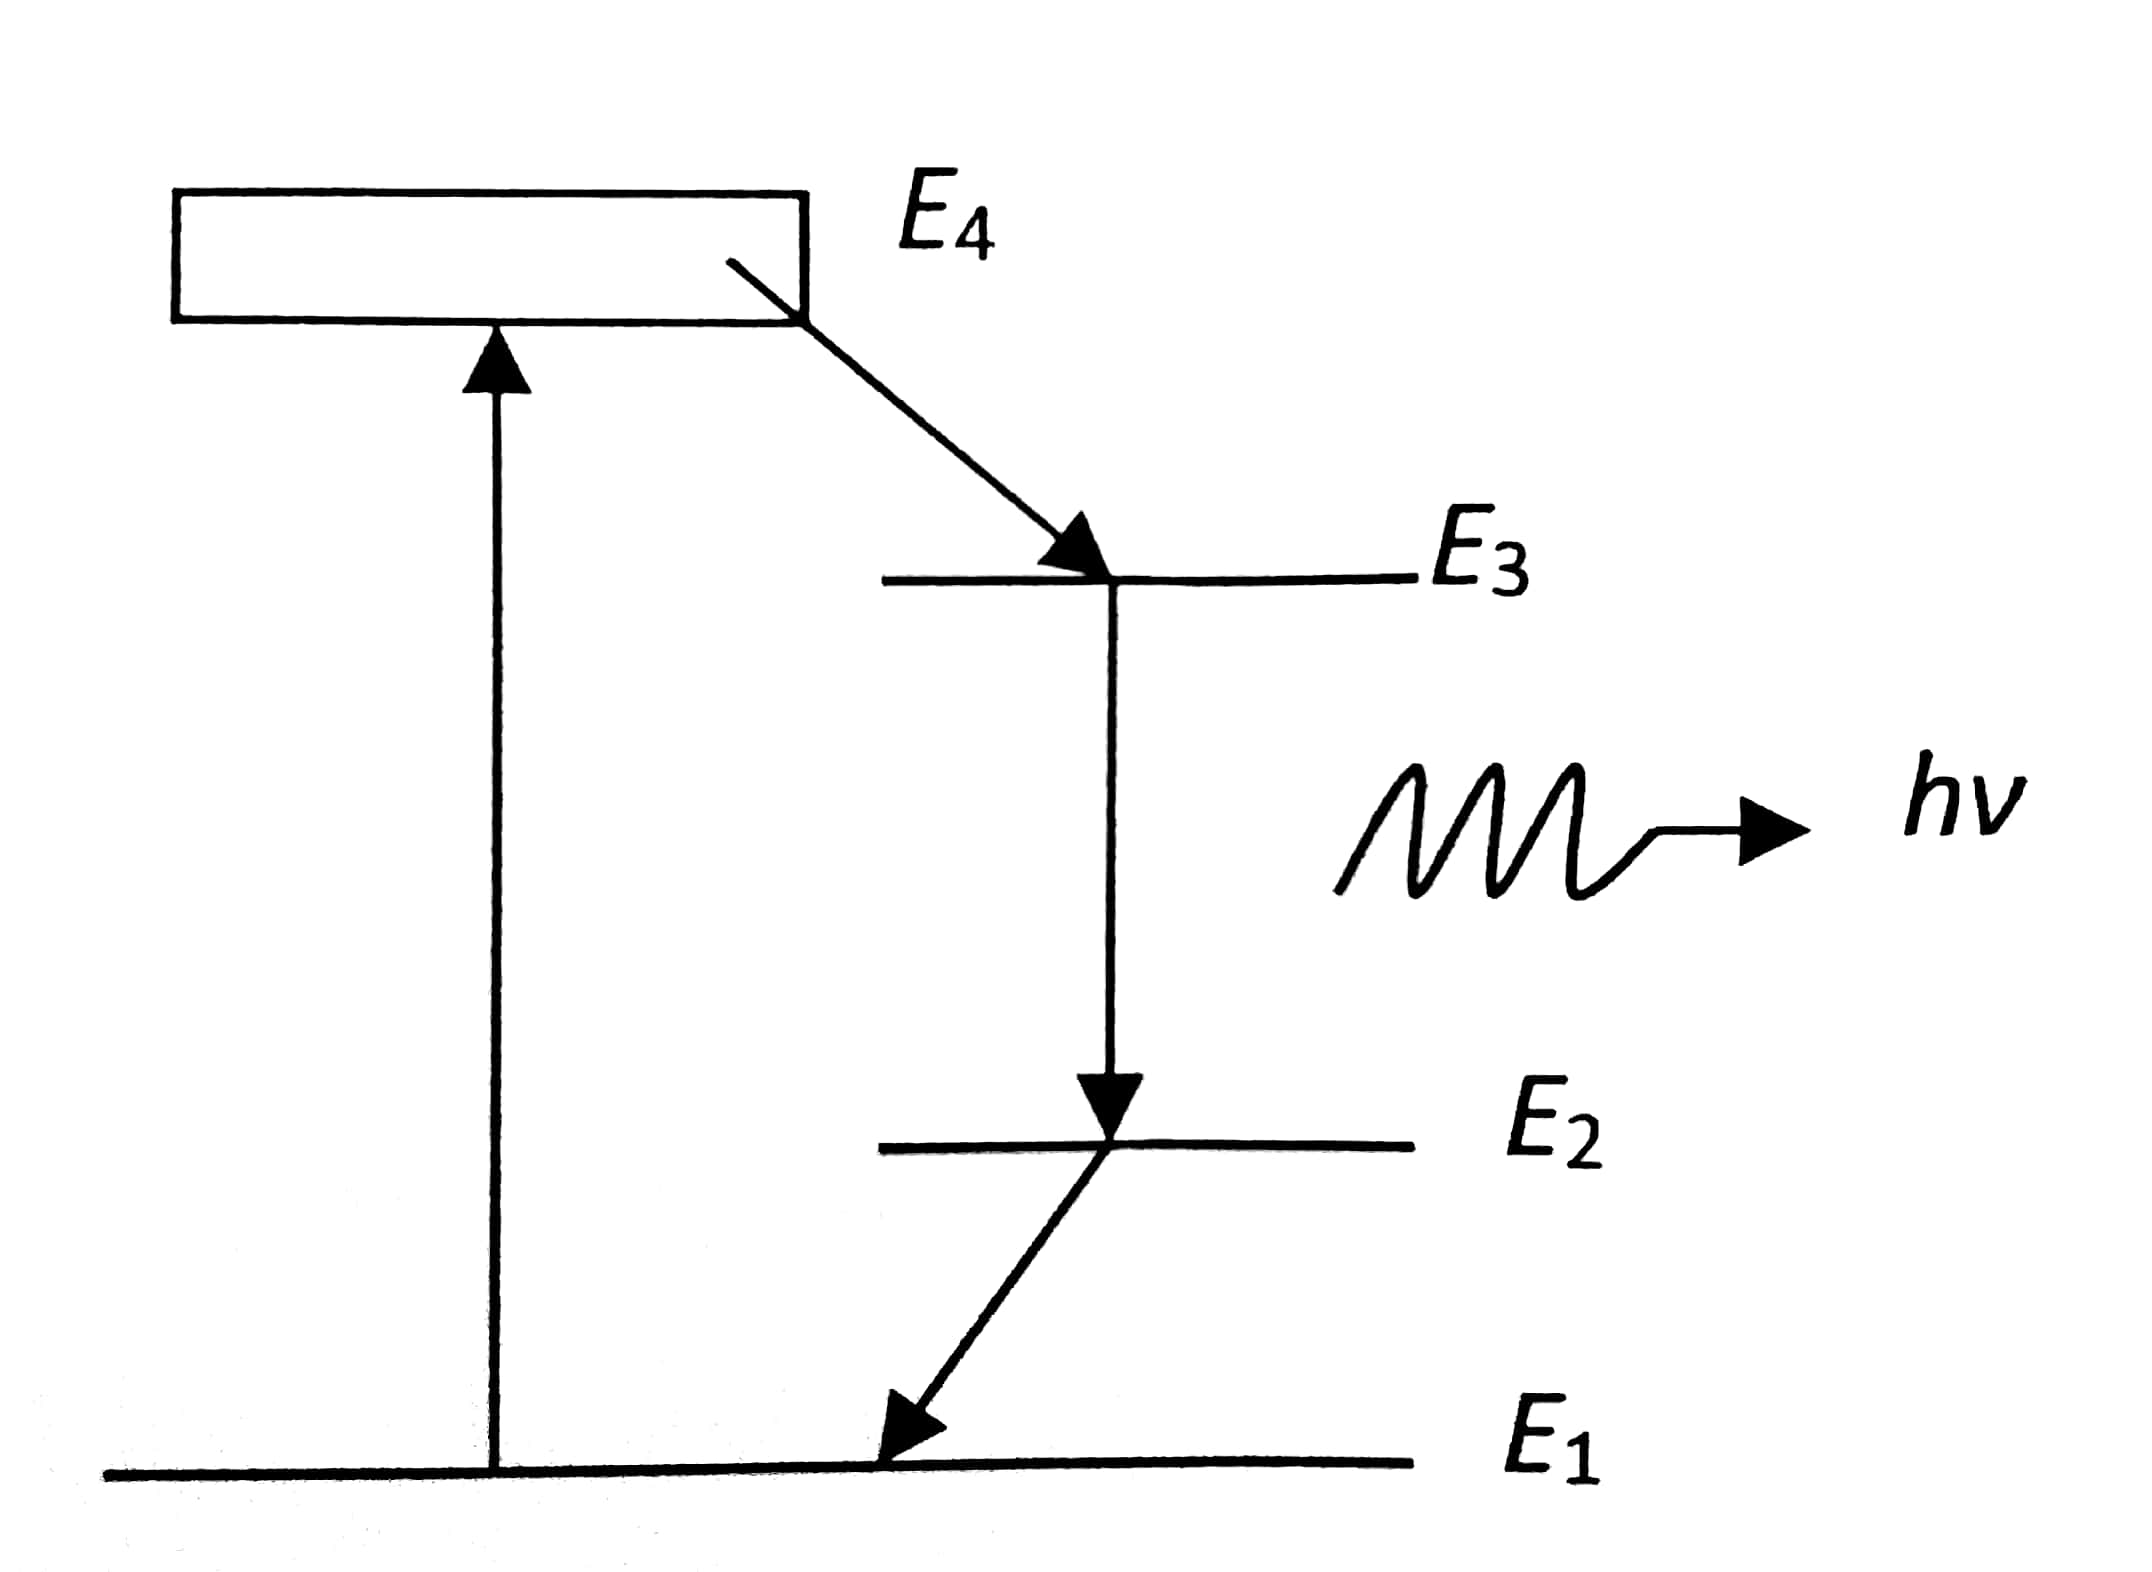
\includegraphics[height=3cm,width=4cm]{images/2.jpg}
    \label{fg2}
  \end{figure}
  \begin{itemize}
    \item 在光泵激励下,钕离子容易在\(\rm E_3\)和\(\rm E_2\)之间形成集聚数反转,实现受激辐射。
    \item 激光器形成自激震荡的条件是\(G^0 \times l \geq \alpha L \)
    \item 静态激光器输出的光脉冲为一群尖峰脉冲序列,称为激光弛豫震荡
  \end{itemize}
  
\end{frame}
\begin{frame}{调Q工作原理}
  \begin{itemize}
    \item 静态激光器因为弛豫震荡,输出功率受到限制。
    \item 采用调Q技术可以使激光能量集中到单脉冲,峰值功率可达兆瓦以上。
    \item 调Q晶体的吸收系数与入射光强之间的关系为:
    \begin{figure}
      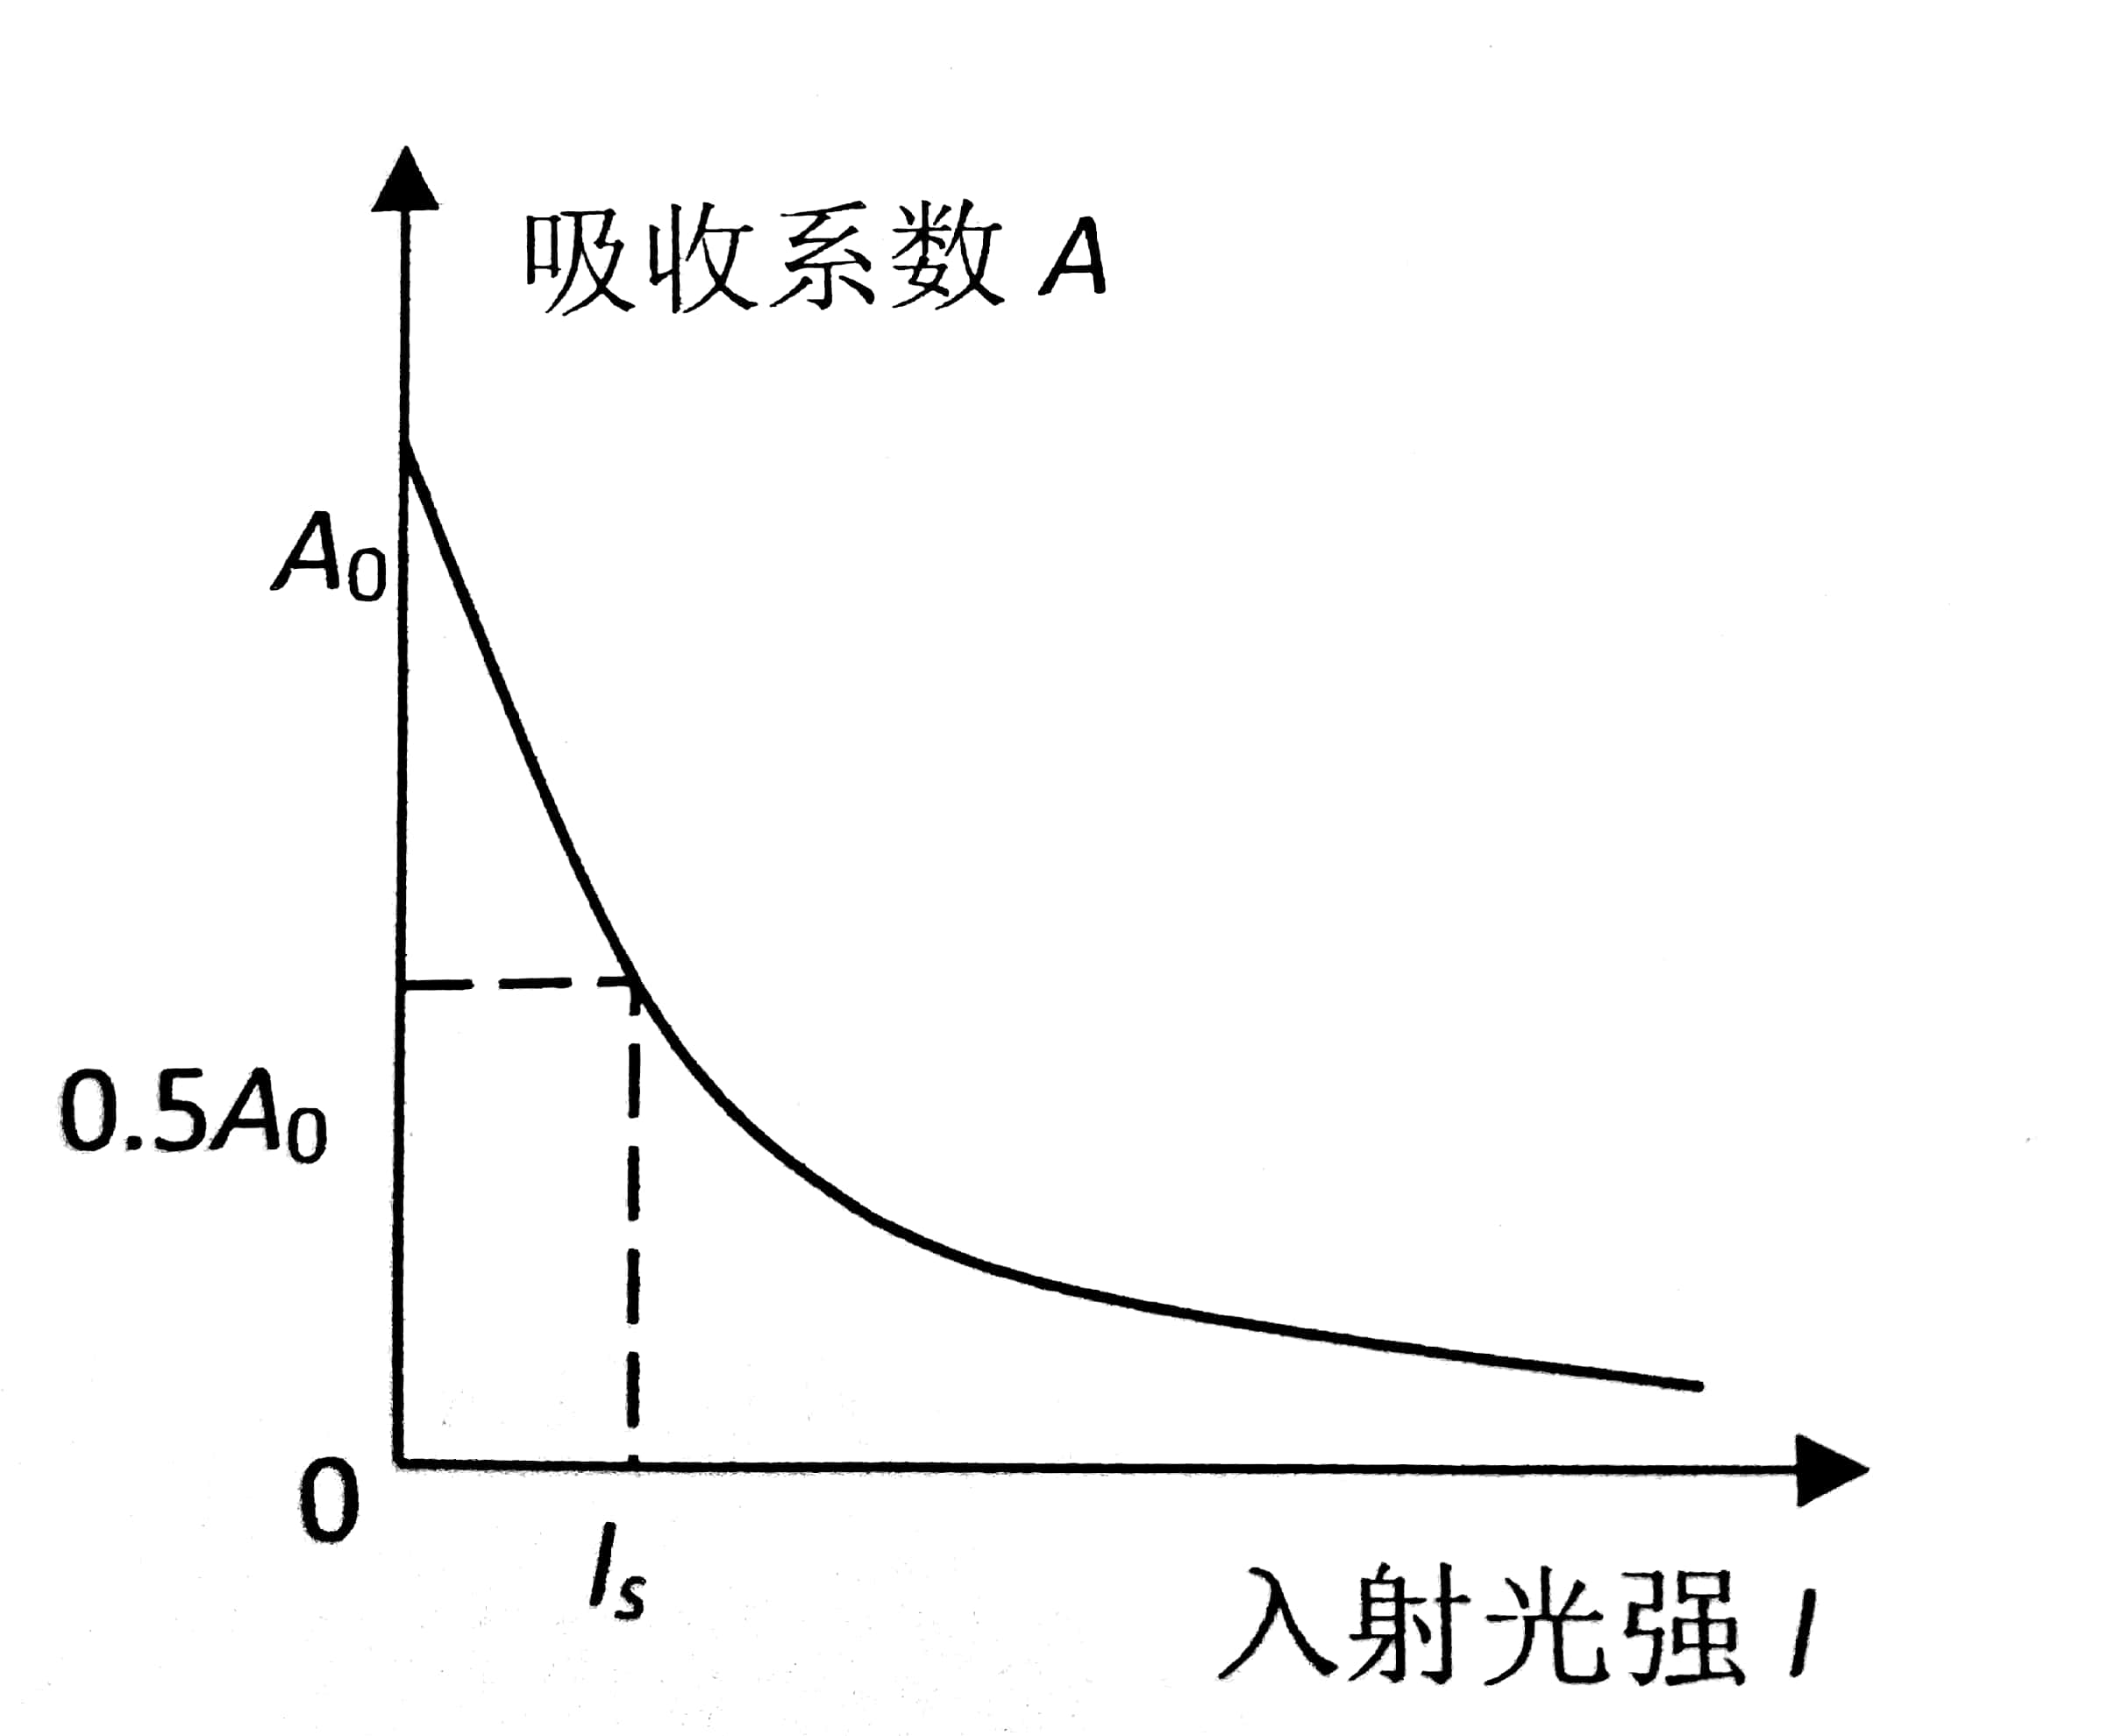
\includegraphics[height=3cm,width=4cm]{images/4.jpg}
      \label{fg2}
    \end{figure}
  \end{itemize}
  


  \begin{itemize}
    \item 光强较弱时,调Q吸收系数大,无法产生激光
    \item 光强增大到一定程度后,调Q吸收系数降低,受激辐射光强急剧增长
  \end{itemize}
  
\end{frame}

\begin{frame}{调Q工作原理}
  \begin{itemize}
    \item 燃料调Q激光器能量输出特性为:
    \begin{figure}
      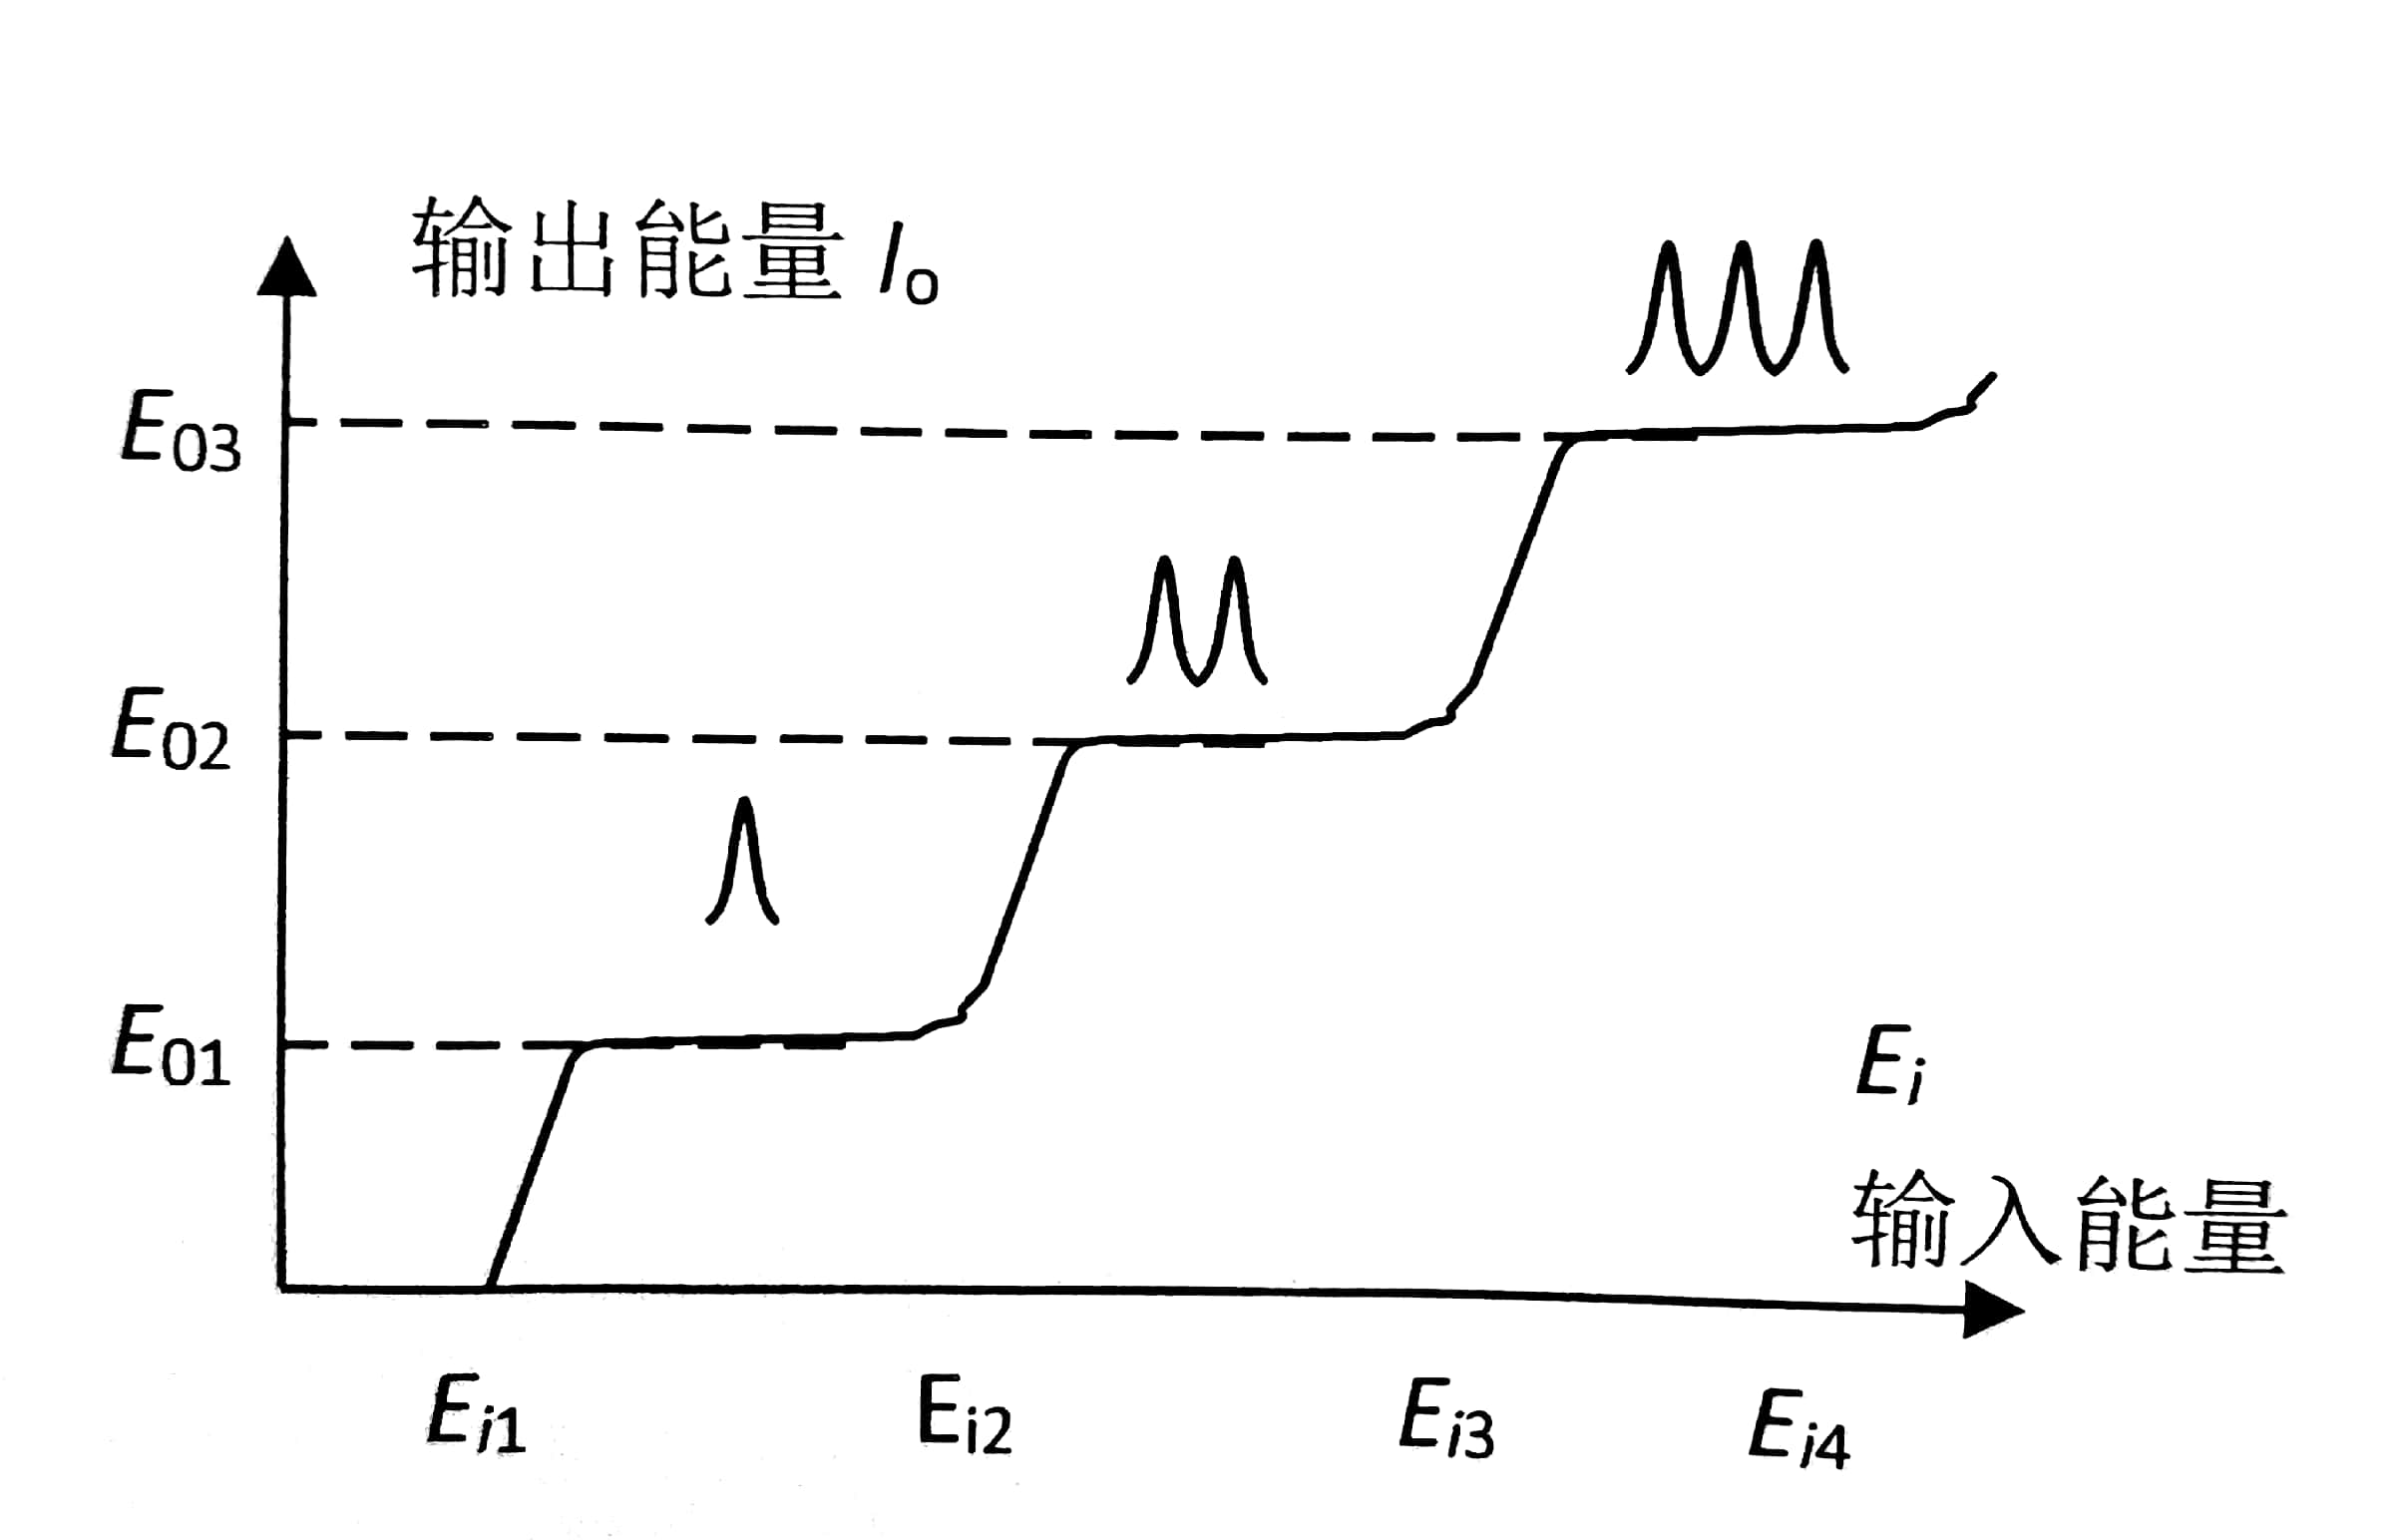
\includegraphics[height=3cm,width=4cm]{images/5.jpg}
      \label{fg2}
    \end{figure}
  \end{itemize}
  

\begin{block}{重要概念}
  \begin{itemize}
    \item 调Q晶体初始透过率
    \item 调Q效率/动静比
  \end{itemize}
\end{block}
  
\end{frame}


%---------------------------------------------------------
% 
%---------------------------------------------------------
\section{实验系统}
\begin{frame}{实验系统}
  \begin{itemize}
    \item 实验装置为:
    \begin{figure}
      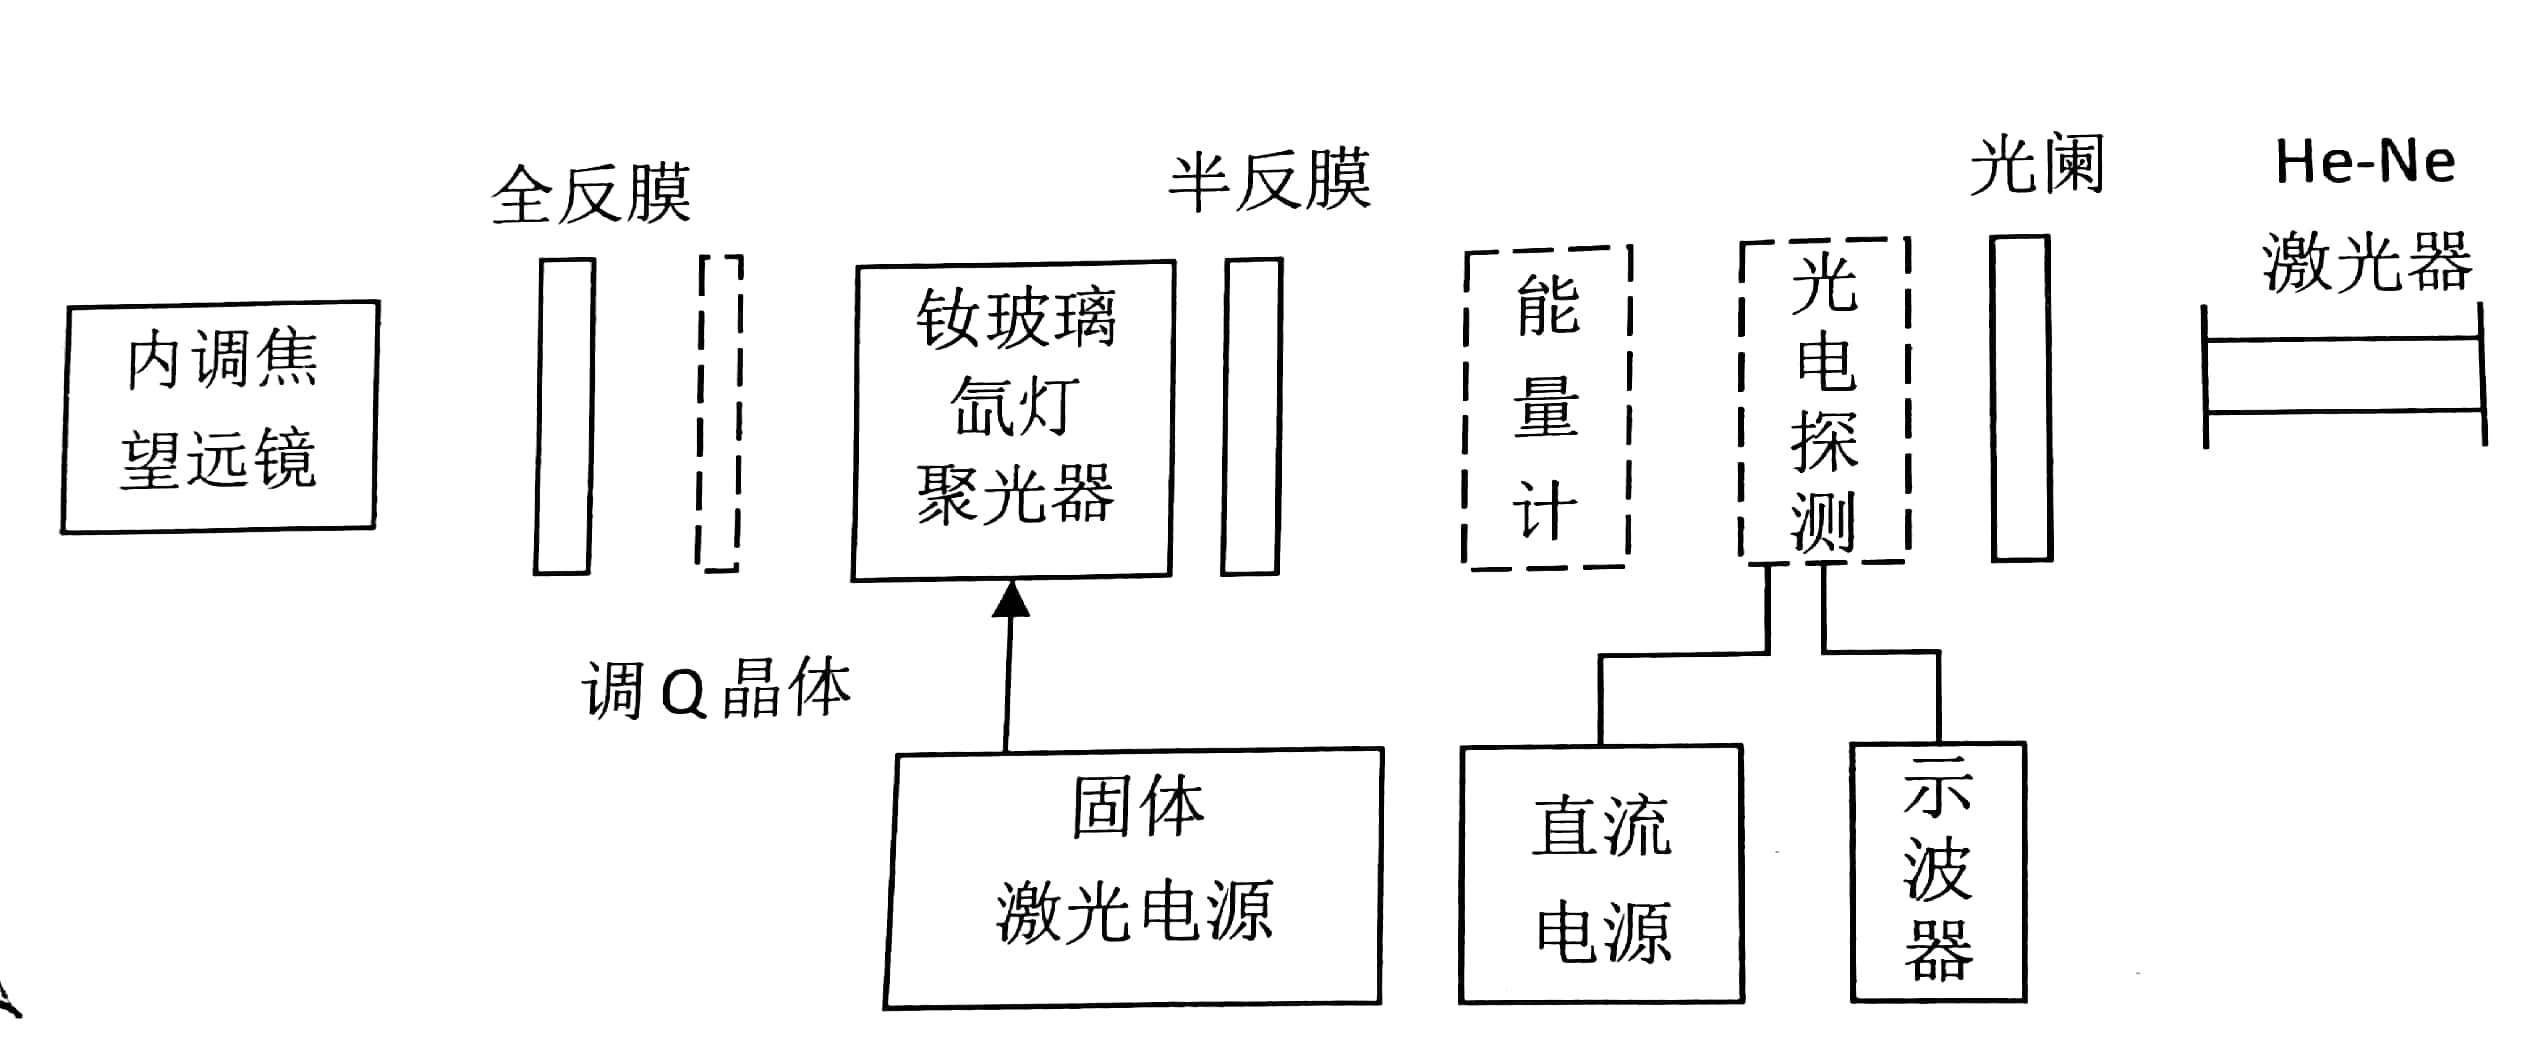
\includegraphics[height=3cm,width=7.5cm]{images/6.jpg}
      \label{fg2}
    \end{figure}
  \end{itemize}
  

\begin{block}{装置简述}
  \begin{description}
    \item[激光器] 分离式结构;采用平行平面腔  
    \item[能量计] 测量脉冲能量
    \item[光电探测器] 灵敏度高,脉冲强激光刺激下饱和,需要加衰减
  \end{description}
\end{block}
  
\end{frame}


\section{方法步骤}
\begin{frame}{光路校准}
  \begin{itemize}
    \item \alert{粗调} 用 He-Ne 激光器准直固体激光器的钕玻璃棒和反射膜片,调整各元件使它们轴向对中并使它们对 He-Ne 激光的反射光斑基本重合
    \item \alert{细调} 用内调焦望远镜细调光路,将各元件调整到严格平行。从望远镜中可以看到几个十字叉丝,其中最亮的叉丝是全反膜反射回来的,最暗的叉丝是半反膜反射回来的,我们只需要调整激光器使得这两个叉丝尽量重合即可
    
  \end{itemize}
\end{frame}
\begin{frame}{激光发射}
  \begin{enumerate}
    \item 将光路调整的比较理想之后,在老师指导下学习固体激光器电源的使用方法,然后发射激光
    \item 测量阈值时,将一张黑纸放置在激光发射口,然后增大输入功率(即电压),直到黑纸上恰好出现白点,此时的输入能量即为阈值
  \end{enumerate}
  本次实验,我们测得的阈值电压为 560V。
\end{frame}
\begin{frame}{数据测量}
\begin{block}{输入输出能量关系曲线}
  \begin{itemize}
    \item 改变输入电压,输入能量可由输入电压换算得到,输出能量用光能量计测量,进而可以画出二者的关系曲线。
  \end{itemize}
\end{block}
\begin{block}{波形观察与参数测量}
  \begin{itemize}
    \item 使用连接示波器的光电探测器观测波形。需对激光进行衰减以避免光强太大导致的探测器饱和失真,先利用纸片进行漫反射,再用光电探测器接收反射信号。
    \item 需要注意必须让示波器位于单次触发模式。由于输出脉冲为正极性,我们应将触发电平调整为正值。
    \item 测量波形宽度,将波形在脉冲处展开,调节横纵坐标尺度得到比较合适测量的波形,再用手动光标进行测量。
  \end{itemize}
 
\end{block}
\end{frame}

\section{实验结果及分析}

\begin{frame}{静态激光器输入输出关系曲线}
  \begin{itemize}
    \item 对实验测量得到的数据进行整理后,绘制出静态激光器输入输出关系曲线如下:
    \begin{figure}
      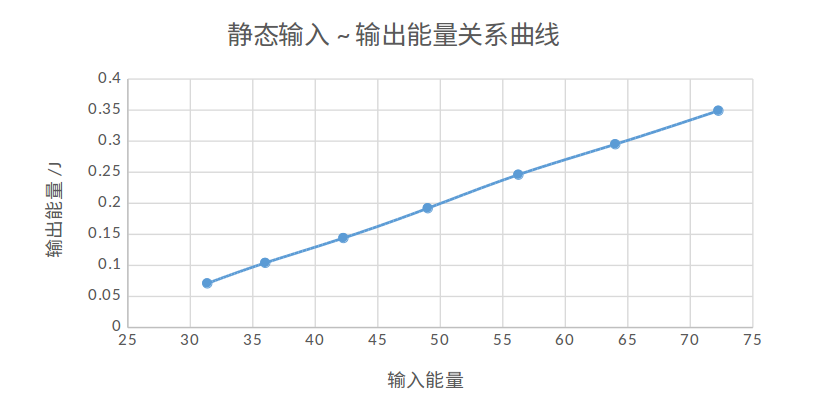
\includegraphics[height=4cm,width=8cm]{images/7.png}
      \label{fg7}
    \end{figure}
    \item 对于静态固体激光器,输出能量与输入能量近似线性变化。这表明当激光器在这一区间工作时,输出能量与输入能量成线性关系。
  \end{itemize}
\end{frame}

\begin{frame}{固体激光器静态输出波形}
  \begin{itemize}
    \item 取输入电压为700V,通过示波器观察驰豫振荡波形并测量其脉冲宽度,实验结果如下:
    \begin{figure}
      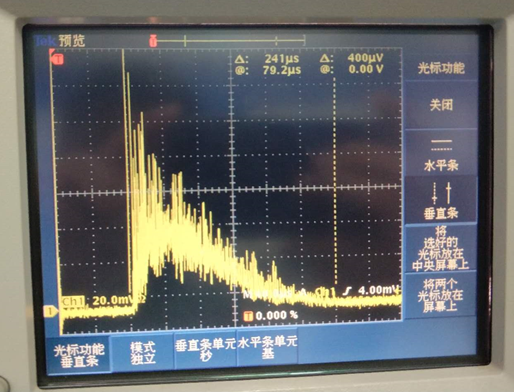
\includegraphics[height=3.92cm,width=5.14cm]{images/8.png}
      \label{fg7}
    \end{figure}
    \item 可以看到确实产生了驰豫振荡,脉冲宽度利用手动光标测量测得约为\(241\mu s\),符合我们的预期。
  \end{itemize}
\end{frame}
\begin{frame}{调Q激光器输入输出能量关系曲线}
  \begin{itemize}
    \item 加入调Q晶体后,我们按照之前的方法重新测量了阈值,得到阈值约为670V,较之前相比有所提高。整理得到的数据,绘制出调Q激光器输入输出关系曲线如下:
    \begin{figure}
      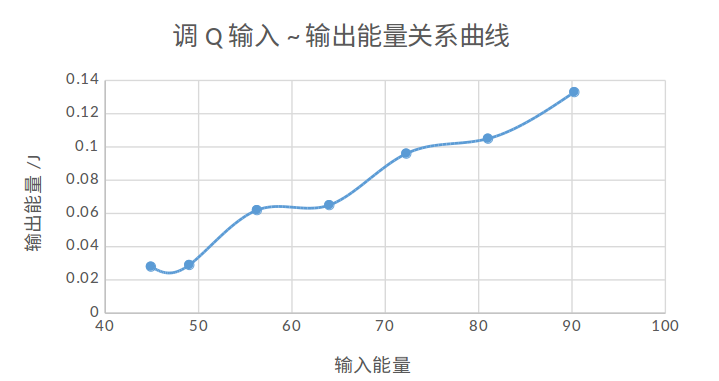
\includegraphics[height=3.8cm,width=7.2cm]{images/9.png}
      \label{fg7}
    \end{figure}
    \item 调Q时输入输出能量关系不再为线性,而是一种类似于阶梯的关系,与我们的理论推算相符。但可能图像采样点太少,阶梯不是太明显。
  \end{itemize}
\end{frame}


\begin{frame}{固体激光器调Q输出波形}
  \begin{itemize}
    \item 添加调Q晶体后,改变输入电压并通过示波器测得此时的输出波形,同时观测脉冲个数,观测结果:
    \begin{figure}[htbp]
      \centering
      \begin{minipage}[htbp]{80pt}
        \centering
        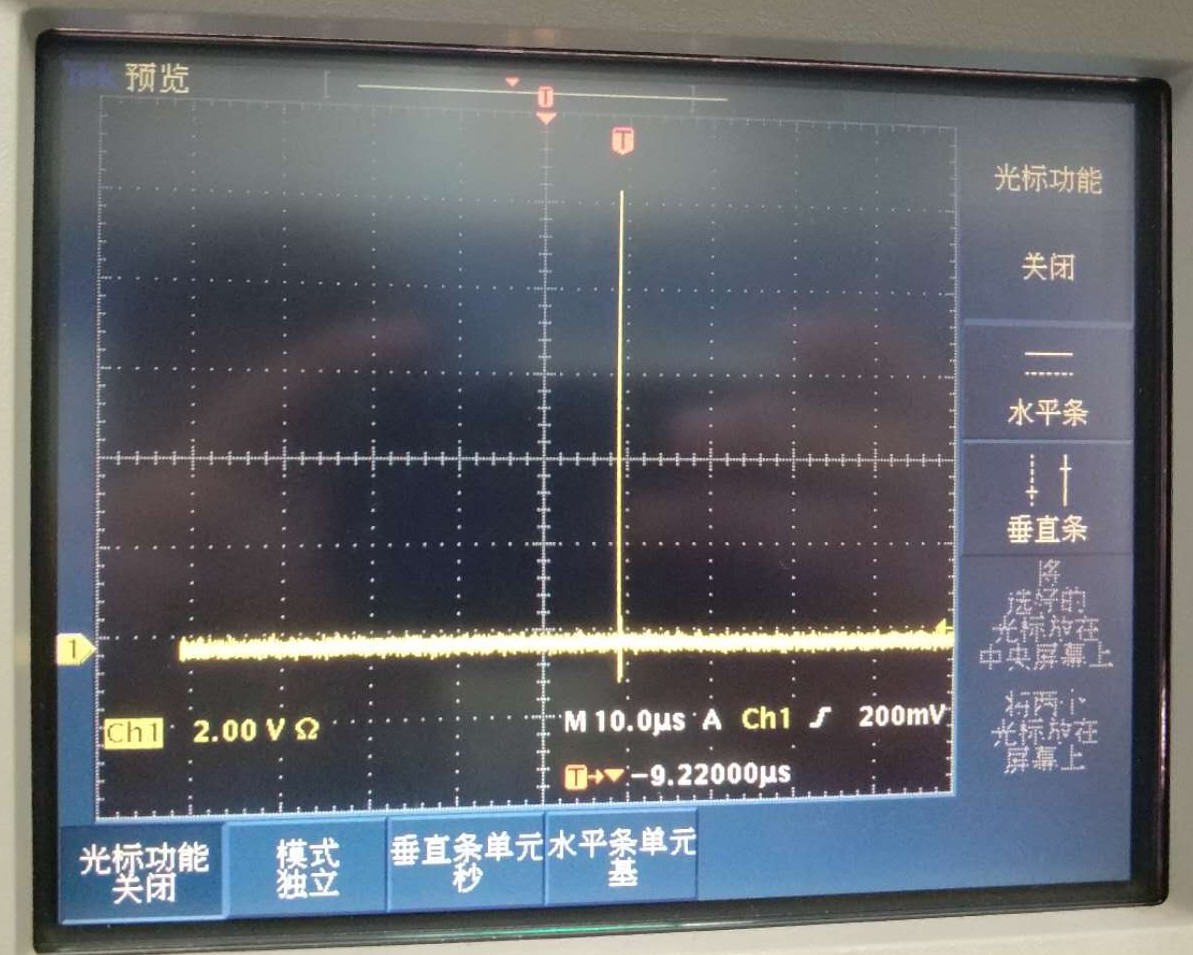
\includegraphics[width=80pt]{images/10.jpg}
        \caption{700V}
        \label{fig:4}
      \end{minipage}
      \hspace{10pt}%
      \begin{minipage}[htpb]{80pt}
        \centering
        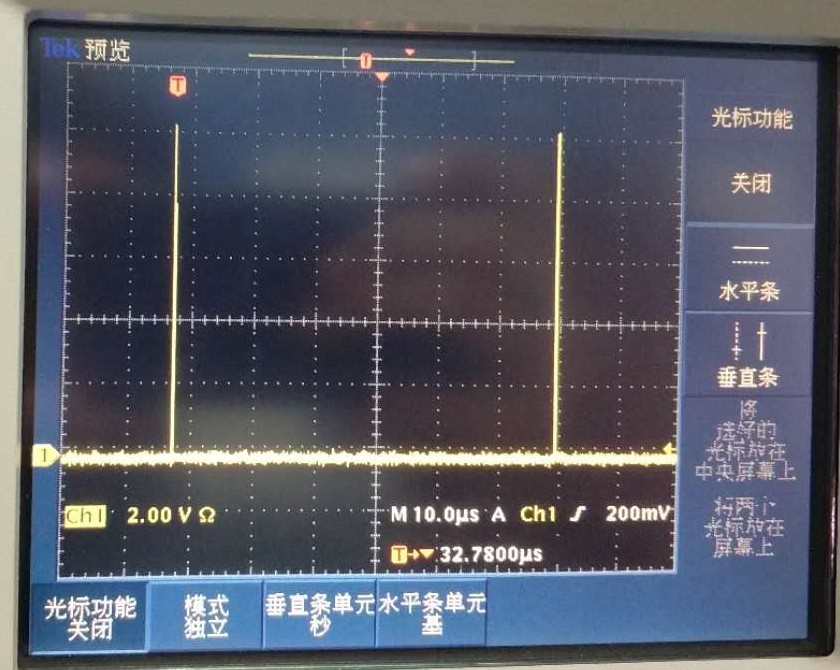
\includegraphics[width=80pt]{images/11.jpg}
        \caption{750V}
        \label{fig:5}
      \end{minipage}
      \hspace{10pt}%
      \begin{minipage}[htpb]{80pt}
        \centering
        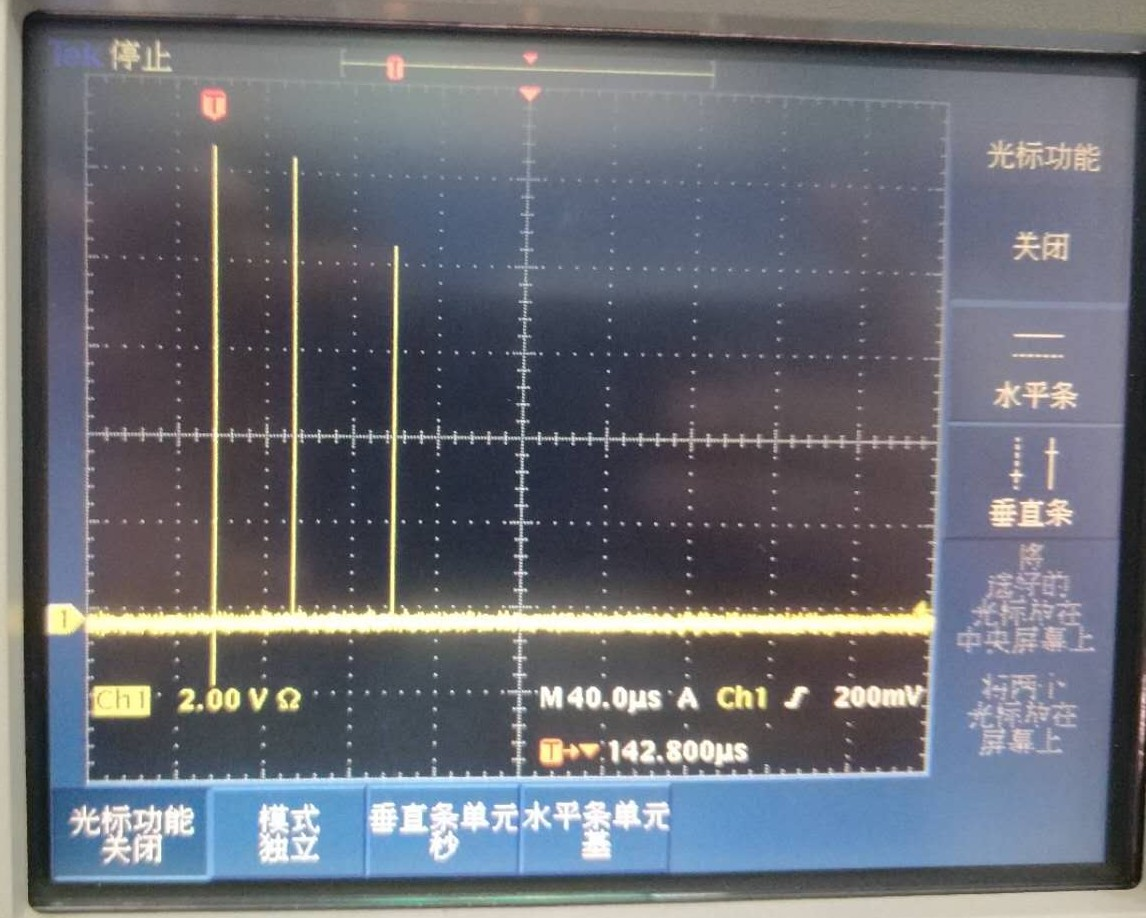
\includegraphics[width=80pt]{images/12.jpg}
        \caption{850V}
        \label{fig:5}
      \end{minipage}
      \end{figure}
    \item 随着输入电压增加,脉冲个数会呈阶梯状提高,应证了我们上一步得到的阶梯曲线。
  \end{itemize}
\end{frame}

\begin{frame}{调Q激光器输入输出能量关系曲线}
  \begin{itemize}
    \item 将 700V时的波形在脉冲处展开,得到的更加细致的波形为:
    \begin{figure}
      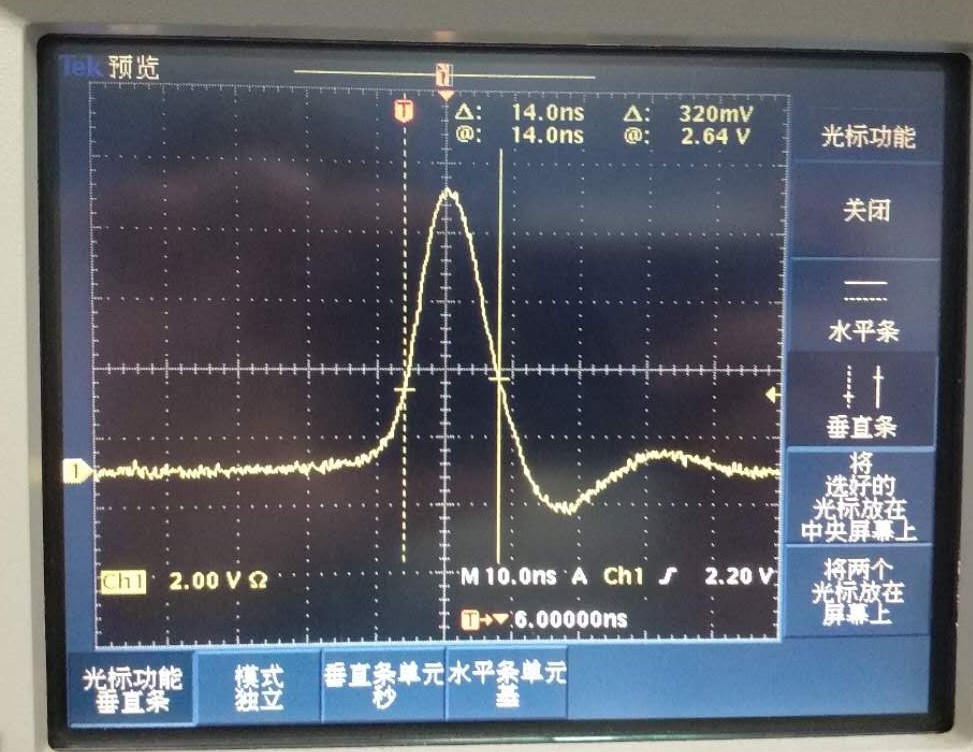
\includegraphics[height=4cm,width=5cm]{images/13.jpg}
      \label{fg7}
    \end{figure}
    \item 调整横纵坐标尺度使得脉冲尽量展开,然后利用手动测量测得单脉冲波形半高全宽约为14ns,符合我们的理论预期
  \end{itemize}
\end{frame}
\begin{frame}{谐振腔调制精度对激光器性能的影响}
  \begin{itemize}
    \item 调偏全反膜,通过目测望远镜视野中叉丝偏离的距离来表示角度偏离,取电压为700V,将得到的数据绘制为曲线:
    \begin{figure}
      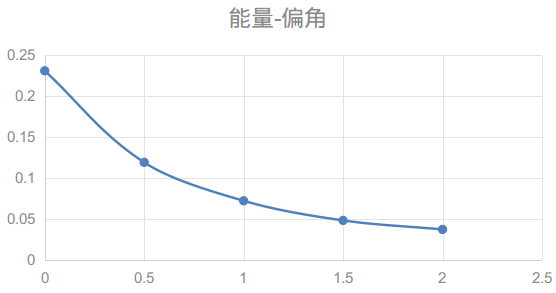
\includegraphics[height=3cm,width=5.5cm]{images/14.png}
      \label{fg7}
    \end{figure}
    \item 在固定输入能量的情况下,随着谐振腔的偏差,输出能量衰减,且开始时衰减得更剧烈。由于我们取的步长太大,这里并没有表现出微调时的结果。
  \end{itemize}
\end{frame}


\begin{frame}
    \begin{figure}
      
\includegraphics[height=2.23cm,width=4.29cm]{images/thank.jpg}
      \label{fg7}
    \end{figure}
   
\end{frame}
\end{document}


% In this slide, some important text will be
% \alert{highlighted} beause it's important.
% Please, don't abuse it.

% \begin{block}{Remark}
% Sample text
% \end{block}

% \begin{alertblock}{Important theorem}
% Sample text in red box
% \end{alertblock}

% \begin{examples}
% Sample text in green box. "Examples" is fixed as block title.
% \end{examples}

%---------------------------------------------------------
%Two columns
% \begin{frame}
% \frametitle{Two-column slide}

% \begin{columns}

% \column{0.5\textwidth}
% This is a text in first column.
% $$E=mc^2$$
% \begin{itemize}
% \item First item
% \item Second item
% \end{itemize}

% \column{0.5\textwidth}
% This text will be in the second column
% and on a second tought this is a nice looking
% layout in some cases.
% \end{columns}
% \end{frame}